\chapter{Distributed Hash Table System} \label{Distribution}

This chapter covers designing \DHTS, a distributed hash table system based on the implemented \PHT class.

\section{Overview}

    \DHTS (DHTS) utilizes a network of \Nodes which run the provided multithreaded application.
    Since the application is symmetrical and decentralised, each \Node has the same set of responsibilities as its peers, and none of the \Nodes is distinguished as a coordinator or a supervisor.

    The system operates on \textit{Persistent Hash Table}, dividing its key-value pairs between the \Nodes.
    Each \Node stores its \PHT fragment locally and can \iterateMethod over it.
    The copy of this fragment is kept by some of the node's peers as a part of the replication process. 
    The number of redundant copies is determined by the \textit{replication factor}.
    
    The \Nodes can operate on the \PHT performing operations such as \insertMethod, \getMethod and \removeMethod.
    To simplify the process of distributing data the \Nodes are organised into a logical ring.
    This way the \textit{consistent hashing} mechanism can be used.
    
    The implemented application provides an administrative console which allows user to manually perform actions (\insertMethod, \getMethod, \removeMethod, \iterateMethod) on the \PHT distributed between \Nodes, list all known \Nodes and test whether another \Node is connected to the network.
    % It also can be used to bulk insert, get and remove sample data for testing purposes.
    
\section{Implementation details}
    \subsection{Decentralised and symmetrical network}
        In a centralised system the coordinator would be responsible for distributing data between the \Nodes. 
        In such an approach the \Nodes' role reduces to performing simple \PHT operations on their local fragments of the \textit{Persistent Hash Table}.
        However, in such an implementation the crash of the master unit causes the entire system to malfunction.
        
        To provide robust fault-tolerance, we decided to implement DHTS in a decentralised manner what has several consequences for the application structure.
    
        Decentralisation implies that no single master controls the data flow in the system.
        This requires the \Nodes to be autonomous and distribute the data themselves.
        To facilitate this, the \Nodes utilise a shared \texttt{hash} method for hashing both \Nodes and hashmap entries.
        Through hashing each \Node is able to independently identify the instance in charge of a specified key.
        
        All the specified requirements result in a higher complexity of the \Node implementation.
        Notwithstanding, it is an insignificant cost compared to the obtained greater system resistance to failures.

    \subsection{Structure}  % listings and description
        The implemented system is composed of several components.

        In order to easily establish and maintain the connection between network participants we provide the \Session class.
        It is a TCP socket wrapper presented in Listing~\ref{SessionListing} which implements the following methods:
        
        \begin{itemize}
            \item \texttt{connect} -- tries to establish a connection on a socket with a \Node listening on the given IP address and port,
            \item \texttt{read} -- wraps async\_read method from \Asio with exception handling; it also serves incoming messages,
            \item \texttt{write} -- wraps async\_write method from \Asio with exception handling,
            \item \texttt{get} -- prepares a get request for a given key and sends it over the socket,
            \item \texttt{insert} -- prepares an insert request for a given key with the provided data and sends it over the socket,
            \item \texttt{remove} -- prepares a remove request for a given key and sends it over the socket.
        \end{itemize}

\begin{figure}[ht] 
\renewcommand{\figurename}{Listing}
    \begin{lstlisting}
template <class K, class V>
class Session {
    tcp::socket socket;
    
    public:
        Session(tcp::socket socket);
        void connect(std::string address, std::string port);
        void read();
        void write(std::string message);
        void get(K key);
        void insert(K key, V value);
        void remove(K key);
}
\end{lstlisting}
\caption{The Session class}
\label{SessionListing}
\end{figure}

The core class is called \Node and is presented in Listing~\ref{NodeListing}. 
It is responsible for spawning threads from the \std namespace, each of which asynchronously accepts connections using the \texttt{accept} method.
For every incoming connection, an object of the \Session class is created and added to the pool of listening sockets.
The class uses \texttt{io\_context} object from \Asio library to handle \texttt{epoll} on Linux.

\begin{figure}[ht] 
\renewcommand{\figurename}{Listing}
\begin{lstlisting}
template <class K, class V>
class Node {
    boost::asio::io_context &io_context;
    short port;
    
    public:
        Node(boost::asio::io_context &io_context, short port);
        void start();
        void accept();
}
    \end{lstlisting}
\caption{The Node class}
\label{NodeListing}
\end{figure}
        
Since \textit{consistent hashing} mechanism is one of the main project assumptions, each \Node has to be familiar with its peers.
For this purpose the \KnownNode class is provided. 
It represents other network participants and is described in Listing~\ref{Node}.
Each \KnownNode object consists of its own address and port as well as a pointer to the \Session object associated with the connection between itself and the \Node.
It also stores Unix epoch time in milliseconds of the moment when connection was established.
Additionally, each \KnownNode has a hash value assigned. We discuss how the hash is computed later.

\begin{figure}[ht] 
\renewcommand{\figurename}{Listing}
    \begin{lstlisting}
class KnownNode {
    public:
        std::string addr;
        std::string port;
        Session *_session;
        int32_t hash;
        long timestamp;

        KnownNode(Session *_session, std::string address,
                      std::string port, std::int32_t hash);
}
    \end{lstlisting}
    
\caption{The KnownNode class}
\label{Node}
\end{figure}

        All \texttt{KnownNodes} are stored in a simple hash map called \NodesMap.
        To this end we use an \texttt{unordered\_map} \cite{Unordered} from the \std namespace.
        
        
        All \texttt{KnownNodes} are stored in a simple hash map called \NodesMap.
        To this end we use an \texttt{unordered\_map} \cite{Unordered} from the \std namespace.
    name space which is an associative array storing key-value pairs.
        It provides basic operations such as \texttt{insert}, \texttt{find} or \texttt{erase} and therefore allows us to keep information about all \texttt{KnownNodes}.
        Since the \texttt{unordered\_map} requires the entries' keys to be unique, they are composed of the \texttt{KnownNode's} IP address concatenated with its port. 
        Each entry's value is an object of \KnownNode type.
        
        \tk{This paragraph is difficult to understand}
        Moreover, the application provides an array of pointers to \PHT used by \Node.
        The array is called \texttt{PMap} and its size depends on the \textit{replication factor}.
        If equal to one, there is only one entry in the array which represents \PHT fragment stored locally by the \Node.
        Next indexes in the \texttt{PMap} array stand for replicas of the next \Node neighbours.

    \subsection{\Asio used methods}
        As described in Section~\ref{Background}, the \DHTS implementation is based on \Asio library.
        Methods are basically generic depending on used protocol and wanted use case.
        \begin{itemize}
            \item \texttt{connect} - establishes connection with TCP socket.
            \item \texttt{async\_accept} - asynchronously accepts a new connection into a socket.
            \item \texttt{async\_read} - asynchronously reads number of bytes of data from socket stream.
            \item \texttt{async\_write} - asynchronous writes a certain number of bytes of data to a socket stream.
        \end{itemize}
        
                
    \subsection{Consistent hashing} \label{ConsistentHashing}
        In order to place all \Nodes on the hash ring, they have to be mapped to a circle.
        As mentioned earlier, each \texttt{Node's} key is represented by a string composed from its IP address and its port. 
        We use the same method to compute the \texttt{Node's} hash as in case of \texttt{SegmentObject's} in \PHT (Listing~\ref{Hash}).
        The only difference lies in the \texttt{range} parameter: for \Nodes it is set to 360 representing an angle of the circle.
            
        Using the same method allows us to easily place both the \PHT data and \Nodes on the same logical hashing ring.
        Position on ring is calculated by hashing key for data and hashing address multiplied by port for \Nodes.
        Each key is assigned to \Node with minimally bigger hash than the hash of the key.
        If no \Node is found, the key is assigned to the \Node with the smallest hash to ensure the continuity of the ring.
            
        The same algorithm is used to find further \Nodes which are responsible for replicating the data represented by this key.
        This approach simplifies the process of redistributing existing data when new \Node joins the system.
        It only requires to change the location of the keys which hashes are assigned to the new participant or are replicated by its closest ring neighbours, leaving the remaining structure intact.
        
    \subsection{Communication protocol}
        \Nodes in \DHTS communicate by sending messages through TCP connections. 
        Each message is a byte array composed of message type, timestamp and data separated by special character. 
        To ensure proper operation of the system, complex generic types used in \PHT has to provide it's on serialising and deserialising methods which will convert data to byte array and back.
        \begin{itemize}
            \item \texttt{connect} -- message is sent after \Node establishes connection with any other member of the network, it contains information about port on which \Node is accepting new connections; when read, a \Node creates new object of \KnownNode with information about connection, then it sends a nodes message; after that \Node calculates which elements from his local \PHT fragment should be stored in new member of the network (based on theirs position on hashing ring) and sends them over; then \Node determines if new participant should be his replicator, if so the whole local \PHT fragment is sent
            \item \texttt{nodes} -- message is sent as a response to connect message, it contains information about every known node stored in \NodesMap; when read, reader adds every \Node to \NodesMap and tries to connect to those which are not yet connected,
            \item \texttt{get} -- message is sent when \Node requests access to data with a specified key; when read, a \Node determines if its hash is associated with \texttt{Node's} position on the hash ring, if it is the \Node access an instance of \PHT to get the data; if data is found it is returned as a part of a result message otherwise result message contains an information that element was not found; if \Node states that key's hash is not associated with \texttt{Node's} position on the hash ring, message is redirected to appropriate \Node,
            \item \texttt{insert} -- message is sent when \Node wants to insert data with a specified key; when read, a \Node determines if its hash is associated with \texttt{Node's} position on the hash ring, if it is the \Node access an instance of \PHT to insert the data; result message contains information about insertion status; if \Node states that key's hash is not associated with \texttt{Node's} position on the hash ring, message is redirected to appropriate \Node,
            \item \texttt{remove} -- message is sent when \Node wants to remove data with a specified key; when read, a \Node determines if its hash is associated with \texttt{Node's} position on the hash ring, if it is the \Node access an instance of \PHT to remove the data; result message contains information about removal status; if \Node states that key's hash is not associated with \texttt{Node's} position on the hash ring, message is redirected to appropriate \Node,
        \end{itemize}
        

\section{Conflict resolutions}
    Every message contains a clock based on Unix time in milliseconds.
    It is used to resolve conflict in situation when \Node disconnects and reconnects to system before information about his absence is acknowledged by everyone in the system.
    If message stating that \Node is disconnected arrives after connection message, it is ignored.

\section{Connection of the hashmap to the node}
    Each \Node operates on local instance of \PHT which represents a fragment of data stored in \DHTS.
    Considering that NVM is emulated in file system each \Node creates a file which is used to save data to ensure its persistence.
    Upon request either from another \Node or keyboard input, \PHT interface is used to access the data.
    Thanks to PHT's support for concurrency, multiple data accesses can be conducted efficiently at the same time without a need of implementing locks.

\section{Evaluation}

    \subsection{Test environment}
        In order to accurately evaluate the implemented \DHTS we had to run several program instances in the same environment.
        Since both \Node and \texttt{PHT} uses all available threads on a current machine, running multiple program instances on the same working station could result in ineffective performance measurements.
        We had to conduct the distribution tests on multiple homogeneous machines, therefore we decided to use the \textit{High Performance Computing} units provided by Poznan University of Technology. 
        
        by the memory size. We conducted tests using the following:
    \begin{itemize}
        \item 4-core processor Intel Xeon X3230 CPU@2.6GHz, % 0.8 GHz - 3.6 GHz,
        \item RAM: 4 GB,
        \item RAM for NVM emulation: 512 MB,
        \item Operating system: Fedora Linux 27
    \end{itemize}
    
        The described project is based on several libraries, whose building process is both complicated and time-consuming.
        To fasten the programming environment setup we decided to use Docker \cite{Docker} --- a tool allowing us to create a virtual operating system image based on a description file.
        We had to provide our own \textit{Dockerfile} combining \textit{PMDK} libraries, \textit{NVM} emulation and \textit{boost library}.
        By using docker we could also clone our repository and fully automate the environment setup process.
        
        %todo: na HPC pamiec RAM tylko podpieta emuluje NVM, nie jest persistent 
    
    \subsection{Tests}
    
        To evaluate the performance scalability of the implemented \DHTS we performed several stress tests.
        
        At first, we decided to analyse the situation in which one thread in one \Node inserts a specified number of elements to an existing network. We performed this test in two variants -- with replication factor 1 and 3.
        
        
        In first variant  -- figure~\ref{rf1} each element is inserted once so decrease in time needed to achieve this task can be observed after adding just one \Node.
        It is thanks to distribution of inserted elements between participants.
        The insertion process is accelerating to the point when it reaches minimal time needed by one thread to process the data and send proper messages.
        
        
        In second variant -- figure~\ref{rf3} increase in time needed to achieve this task can be noticed.
        Improvement is directly connected to used replication level.
        If only one \Node is in network it has to insert every element once, but when another \Node is added, every \Node has to insert every element twice -- in a local \PHT fragment and in a replicated \PHT fragment of another \Node.
        A chart reaches peak when number of nodes is equal to replication factor -- every \Node has to insert each element three times.
        Then the time needed for insertion is decreasing thanks to distribution of work.
        Scaling on many \Nodes reaches minimal time needed for one thread to process the data and send proper messages.
        
        
        In second test -- figure~\ref{mrf3}, we analysed the situation in which inserted elements are equally divided between members of the network.
        Input data is processed on one thread on each \Node in opposition to first test where only one thread on one \Node processed the input data.
        Thanks to this, insertion can be completed in less time than previously even though replication factor is set to 3 and every element is inserted three times from the moment when number of \Nodes reaches 3.

    \begin{figure}[ht]
        \centering
        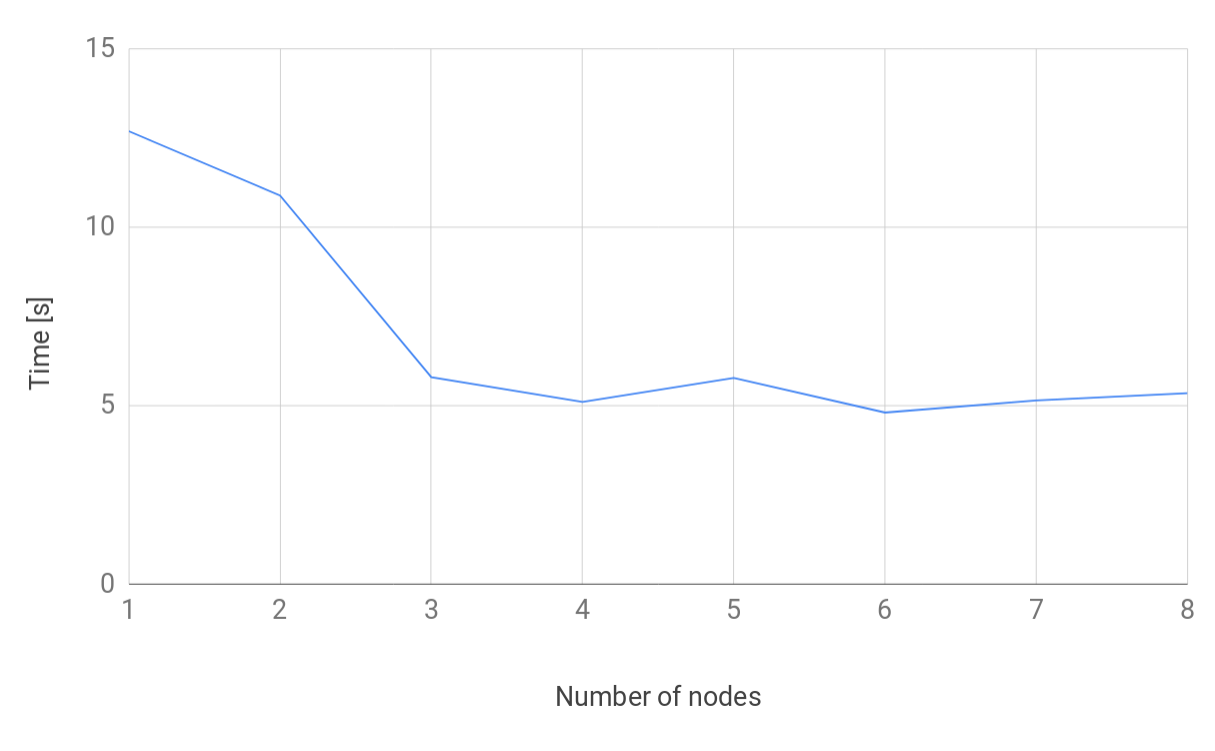
\includegraphics[width=0.8\textwidth]{thesis/figures/rf1.png}
        \caption{Time measurements for inserting 200,000 elements by one \Node with replication factor 1}
        \label{rf1}
    \end{figure}
    
    \begin{figure}[ht]
        \centering
        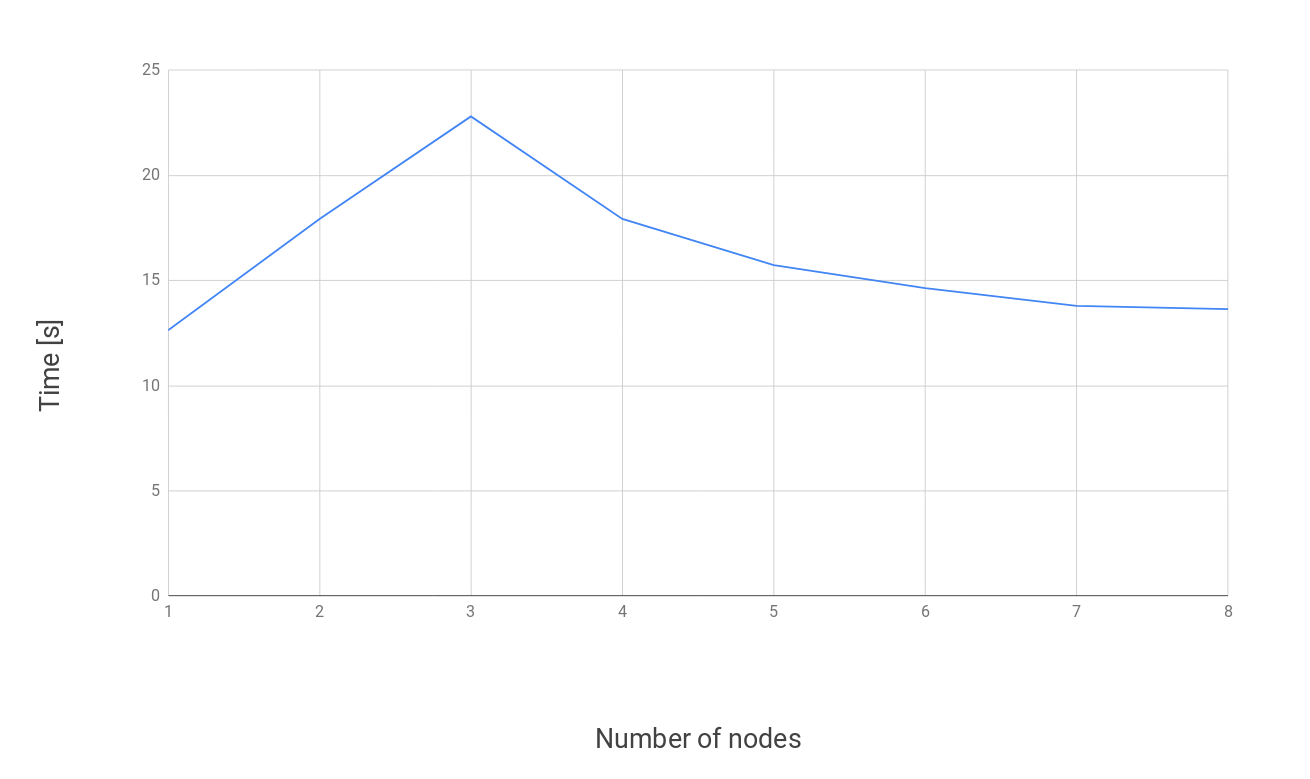
\includegraphics[width=0.8\textwidth]{thesis/figures/rf3.png}
        \caption{Time measurements for inserting 200,000 elements by one \Node with replication factor 3}
        \label{rf3}
    \end{figure}
    
    \begin{figure}[ht]
        \centering
        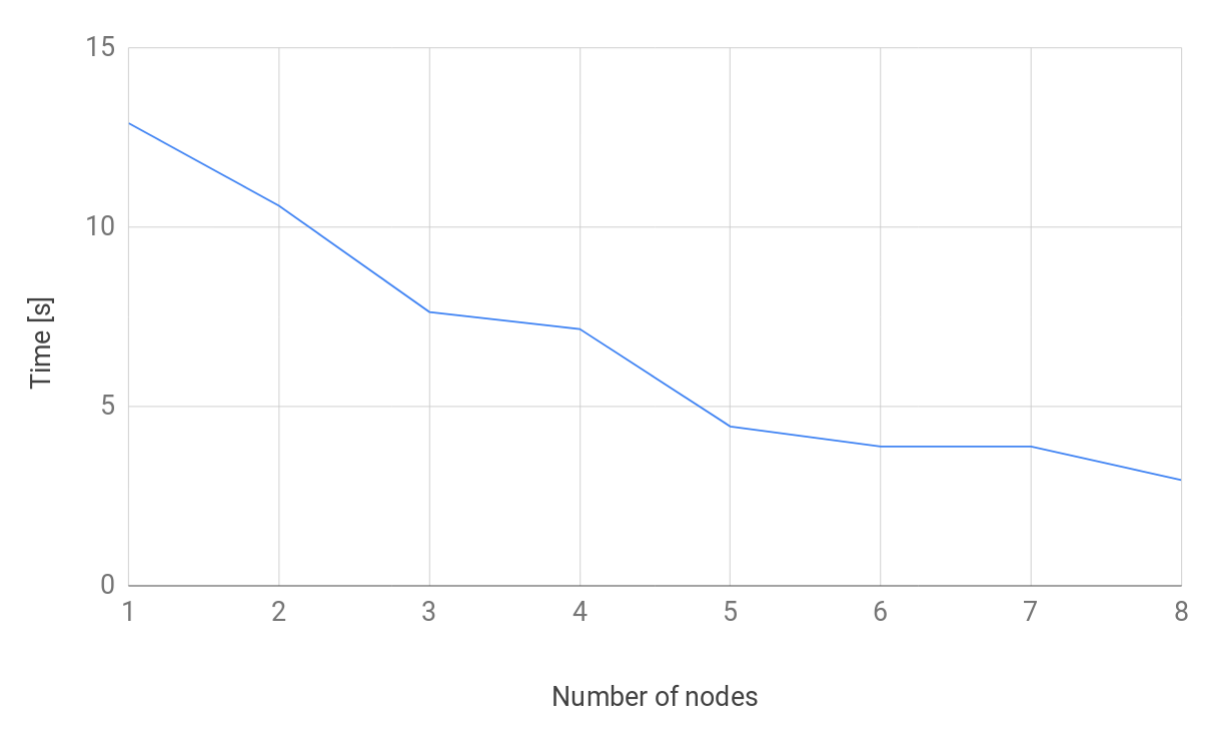
\includegraphics[width=0.8\textwidth]{thesis/figures/rf3MultipleInserts.png}
        \caption{Time measurements for multiple \Nodes inserting 200,000 elements altogether with replication factor 3}
        \label{mrf3}
    \end{figure}
    

\section{Conclusions}
    In this chapter we discussed  \DHTS, a distributed system for the implemented \PHT class.
    Extensive tests allowed us to ensure its correctness and uncover several bugs related to communication process.
    
    
    We managed to build symmetrical and decentralised system in which each participant has the same set of responsibilities and there is no superior unit.
    It provides basic actions necessary to test \PHT such as \insertMethod, \getMethod and \removeMethod.
    We have also implemented consistent hashing and replication mechanisms which are standards modern distributed solutions.
    
    
    Prepared \DHTS implementation allowed us to test scalability of \PHT in distributed environment.
    
    
    The described system provides the major assumptions of the project, however, it leaves room for improvement, especially in failure detection area.